\newcommand{\Title}{Little Robot} 
\title{\Title}

\documentclass[a4paper]{article}
\usepackage{geometry}
\geometry{a4paper,tmargin=25mm,bmargin=35mm,lmargin=20mm,rmargin=20mm,footskip=5mm}
\usepackage[utf8x]{inputenc}
\usepackage{fontspec}
\usepackage{graphicx}
\usepackage{subcaption}
\usepackage{capt-of}
\usepackage[ngerman]{babel}
\usepackage[colorlinks=true,linkcolor=black,urlcolor=black]{hyperref}
\usepackage[headsepline,footsepline]{scrlayer-scrpage}


\usepackage{xcolor,soul}
\usepackage{colortbl} % Farbige Tabellen

\usepackage{longtable}

\pagestyle{scrheadings}
\clearscrheadfoot

\definecolor{LightGray}{rgb}{0.9,0.9,0.9}
\newcommand{\CItoprowcolor}{\rowcolor{LightGray}}

%%Head
\ihead{{\textbf{\large \Title}}}
\ohead{\raisebox{0.1\totalheight}{
\includegraphics[width=0.15\textwidth]{../pictures/wak-lab-LOGO.png}}}

%%Foot
\cfoot{\pagemark}
\ofoot{\today}

\addto\captionsngerman{
\renewcommand{\figurename}{Abb.}
\renewcommand{\tablename}{Tab.}
}

\begin{document}
\maketitle
%\tableofcontents
\begin{center}
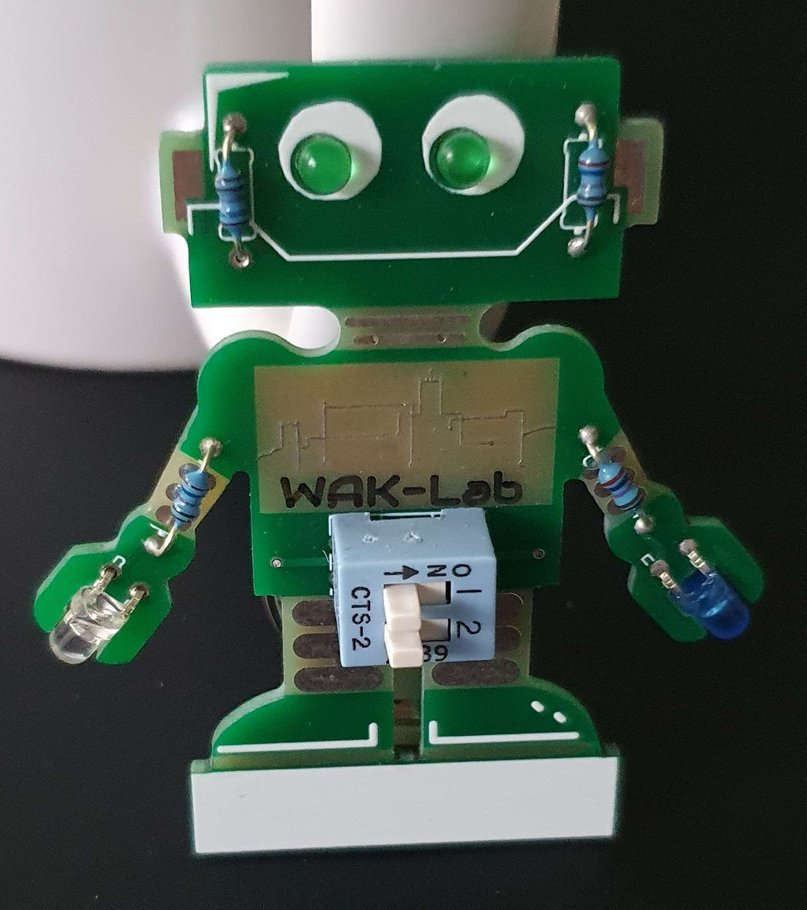
\includegraphics[height=8cm]{../pictures/RoboAus.jpg}
\ \\
\ \\
\ \\
Design: Martin Hildebrandt\\
licensed CC BY\\
\ \\
Logo: By Dorothea Wendt\\
licensed CC BY-ND\\
\end{center}
\newpage
\section{Einleitung}
Der Bausatz ist gedacht als kleine Lötübung für einen einfachen Stromkreis mit  4 LEDs, 2 Schaltern, 4 Widerständen und einer Knopfzelle CR2032.\\
Im Schaltplan sieht man, dass die Spannung am Pluspol der Batterie (3V) erst durch die Schalter muss, dann verzweigen wir auf je einen Widerstand. Die LEDs benötigen etwa 2V, das ist von Farbe zu Farbe unterschiedlich.\\ Es bleibt 1V für die Widerstände übrig. Das Ohmsche Gesetzt $R = \frac{U}{I}$ bzw. umgestellt auf $I = \frac{U}{R}$ lässt uns ausrechnen, dass ein Strom von $I = \frac{1V}{2,7 k\Omega} = 0,37 mA$ pro LED fließt. Das ist wenig, daher werdet ihr lange Freude an eurem Roboter haben.\\
Übrigens: Alle Leitungen die an das Symbol GND gehen, sind untereinander verbunden, damit der Strom weiter zum Minus-Pol der Batterie fließen kann.\\
\ \\
\begin{minipage}[t]{\textwidth}
  \centering
  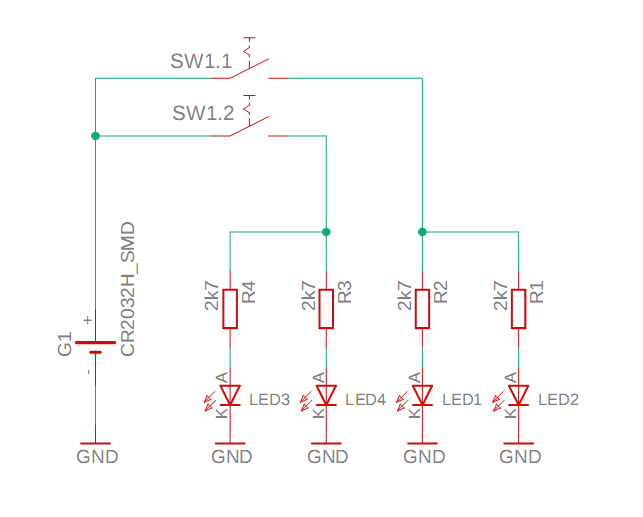
\includegraphics[width=0.55\textwidth]{../pictures/Schematic}
  \captionof{figure}{Schaltplan}
  \label{img:Schematic}
\end{minipage}

\subsection{Kurz etwas zum Löten}
Beim Löten stellen wir eine feste Verbindung aus Metall her. Dazu wird der Lötkolben auf ca. 350$^{\circ}$C eingestellt. Die Bauteile werden beim Löten sehr hei\ss \ und können nicht mit dem Finger gehalten werden (Verbrennungsgefahr). Die Lötspitze darf auch nie den Tisch berühren. Dies hinterlässt hässliche Brandflecken. Der Lötkolben ist immer sicher zu lagern und das Anschlusskabel und die Steckdose sollen sicher verlegt sein (Stolpergefahr).\\
Zunächst wird das Bauteil eingefädelt. Das Beinchen vom Bauteil kann etwas nach au\ss en gebogen werden, damit es fixiert ist. Dann mit dem Lötkolben Pad und Beinchen aufheizen und dann etwas Zinn von der gegenüber liegenden den Seite heranführen und aufschmelzen. Nach etwas 1-2 Sekunden sollte genug Zinn an der Verbindung sein. Die Zeit kann stark variieren, je nach dem, wieviel Wärme von Bauteil oder Pad aufgenommen wird.\\
\ \\
Zum Löten benötigen Wir:
\begin{itemize}
  \item     den Bausatz
  \item     einen Lötkolben
  \item     etwas Lötzinn
  \item     einen Seitenschneider
  \item     eine feuerfeste Unterlage
  \item     optional eine Flachzange
\end{itemize}

\section{Aufbau}
\begin{minipage}[t]{\textwidth}
  \centering
  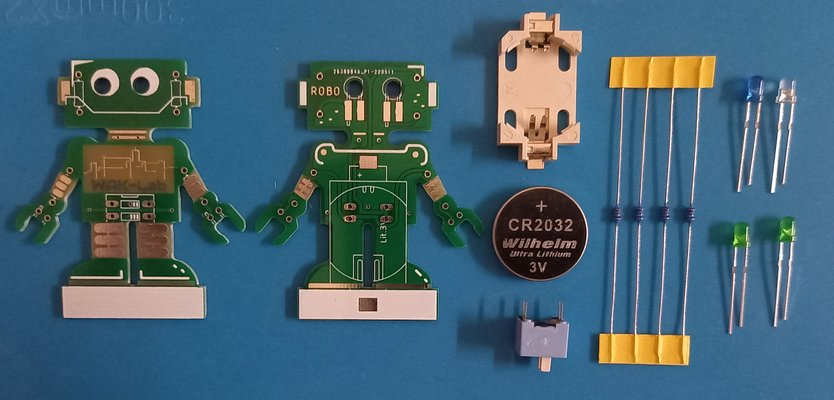
\includegraphics[width=0.9\textwidth]{../pictures/Parts.jpg}
  \captionof{figure}{Bauteile}
  \label{img:Bauteile}
\end{minipage}
\ \\
Bauteile:
\begin{itemize}
\item die Roboter Leiterplatte
\item einen zweifach Dipschalter
\item einen SMD Batteriehalter CR2032
\item eine Lithium Batterie CR2032
\item 4 Widerstände 2,7 k$\Omega$ 
\item 4 farbige LEDs
\end{itemize}
\subsection{Schritt 1 - Widerstände}
Einfädeln der Widerstände von vorne, an den Armen und an den Ohren. An der Rückseite etwas abknicken, damit sie nicht wieder herausrutschen.\\
Dann mit dem Lötkolben die Stelle erwärmen und das Lötzinn dazugeben. Beim ersten Mal schlage ich vor, dass ein erfahrener Löter den Lötkolben nimmt und ihr das Zinn. Danach tauscht ihr. Wenn das gut klappt, könnt ihr mit beiden Händen Zinn und Lötkolben gleichzeitig führen. \\
Am Schluss mit dem Seitenschneider die überstehenden Enden abschneiden.\\
\ \\
\begin{minipage}[t]{0.33\textwidth}
  \centering
  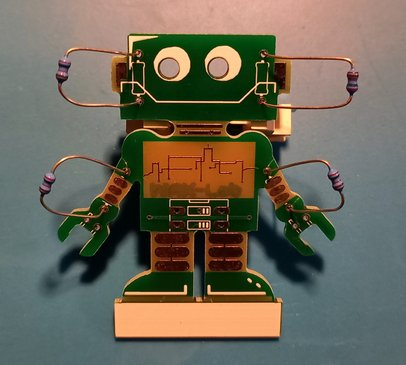
\includegraphics[height=4cm]{../pictures/Resistor1.jpg}
  \captionof{figure}{Widerstände einfädeln}
  \label{img:Resistor1}
  \end{minipage}
\begin{minipage}[t]{0.33\textwidth}
  \centering
  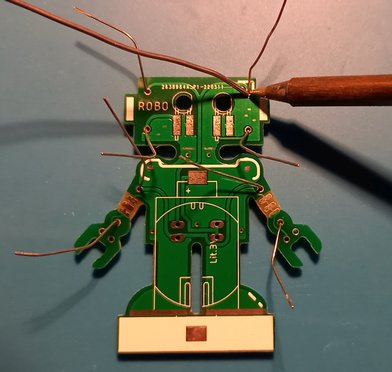
\includegraphics[height=4cm]{../pictures/Resistor2.jpg}
  \captionof{figure}{Widerstände verlöten}
  \label{img:Resistor2}
\end{minipage}
\begin{minipage}[t]{0.33\textwidth}
  \centering
  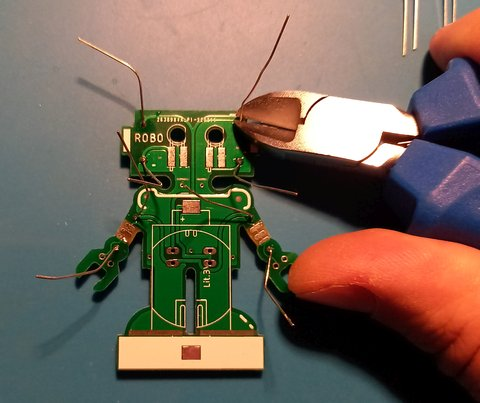
\includegraphics[height=4cm]{../pictures/Resistor3.jpg}
  \captionof{figure}{Beinchen abschneiden}
  \label{img:Resistor3}
\end{minipage}
\subsection{Schritt 2 - Schalter}
Den Schalter stecken wir am Bauch durch die Lötaugen. Auf dem Schalter steht -> ON. Das heißt, dass er nach rechts eingeschaltet wird. Möchte man das anders herum, darf man ihn auch umdrehen.\\
Auf der Rückseite knicken wir die Anschlüsse ganz flach nach unten, bevor wir sie verlöten. Das ist wichtig, damit der Batteriehalter nachher noch darüber Platz hat. Dann verlöten wir ihn so flach wie möglich.\\ \ \\
\begin{minipage}[t]{0.33\textwidth}
  \centering
  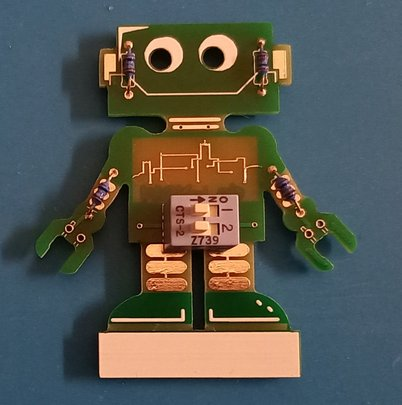
\includegraphics[height=4cm]{../pictures/Switch1.jpg}
  \captionof{figure}{Schalter einsetzen}
  \label{img:Switch1}
  \end{minipage}
\begin{minipage}[t]{0.33\textwidth}
  \centering
  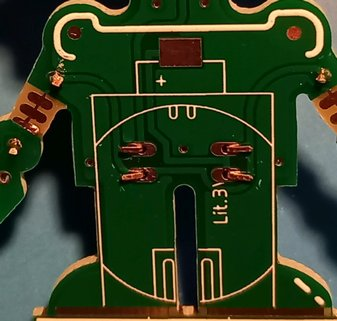
\includegraphics[height=4cm]{../pictures/Switch2.jpg}
  \captionof{figure}{Pins umknicken}
  \label{img:Switch2}
\end{minipage}
\begin{minipage}[t]{0.33\textwidth}
  \centering
  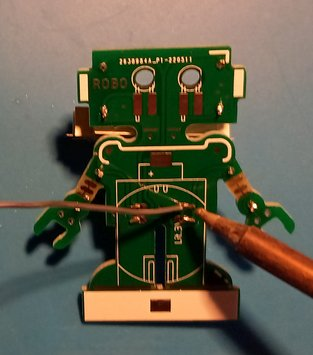
\includegraphics[height=4cm]{../pictures/Switch3.jpg}
  \captionof{figure}{Pins verlöten}
  \label{img:Switch3}
\end{minipage}
\subsection{Schritt 3 - Batteriehalter}
Für den Batteriehalter machen wir vorher schon einen kleinen Klecks aus Lötzinn. Dann lässt sich danach der Halter schöner anlöten, da man den Battierhalter etwas festhalten muss und man keine Hand mehr frei hat für das Zinn. Achtet darauf, dass der Halter richtig herum ist. Vielleicht macht ihr das auch zu zweit und ohne euch zu verletzen.\\
Wenn die zweite Seite angelötet ist, kann man die erste noch etwas nachlöten.\\
\ \\
\begin{minipage}[t]{0.33\textwidth}
  \centering
  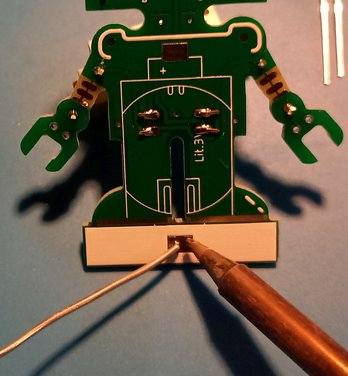
\includegraphics[height=4cm]{../pictures/Bat1.jpg}
  \captionof{figure}{Pad verzinnen}
  \label{img:Bat1}
  \end{minipage}
\begin{minipage}[t]{0.33\textwidth}
  \centering
  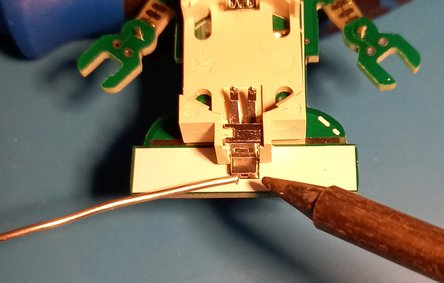
\includegraphics[height=4cm]{../pictures/Bat2.jpg}
  \captionof{figure}{Anschluss anlöten}
  \label{img:Bat2}
\end{minipage}
\begin{minipage}[t]{0.33\textwidth}
  \centering
  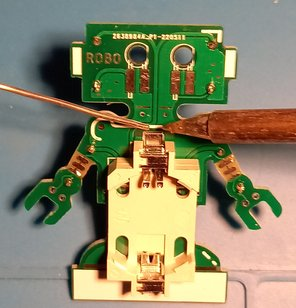
\includegraphics[height=4cm]{../pictures/Bat3.jpg}
  \captionof{figure}{Anschluss anlöten}
  \label{img:Bat3}
\end{minipage}
\subsection{Schritt 4 - Hände}
Die LEDs müssen richtig herum angelötet werden, sonst funktionieren sie nicht: Das lange Beinchen bitte nach rechts, dorthin wo die kleine Markierung am Lötauge ist.\\
Wir stecken die LEDs nicht ganz durch, damit wir sie noch in die Handflächen des Roboters knicken können.\\
\ \\
\begin{minipage}[t]{0.33\textwidth}
  \centering
  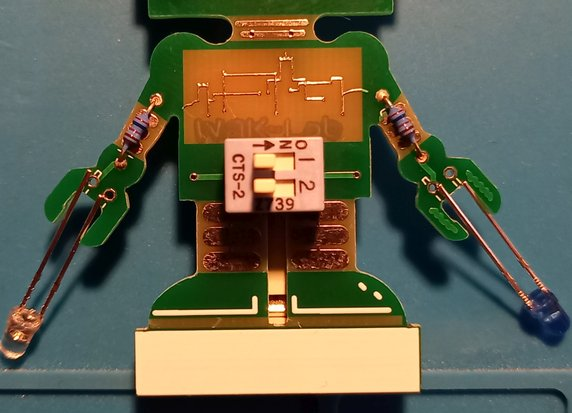
\includegraphics[height=3.5cm]{../pictures/LED1.jpg}
  \captionof{figure}{Richtig einfädeln}
  \label{img:LED1}
  \end{minipage}
\begin{minipage}[t]{0.33\textwidth}
  \centering
  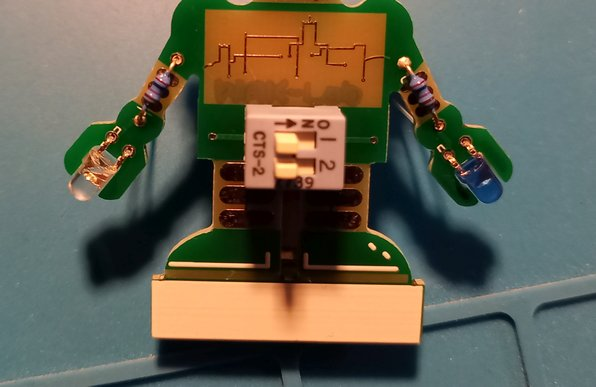
\includegraphics[height=3.5cm]{../pictures/LED2.jpg}
  \captionof{figure}{LED Abknicken}
  \label{img:LED2}
\end{minipage}
\begin{minipage}[t]{0.33\textwidth}
  \centering
  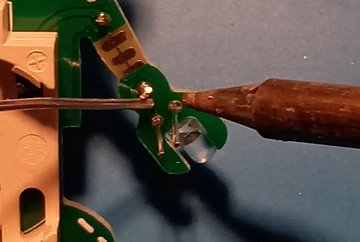
\includegraphics[height=3.5cm]{../pictures/LED3.jpg}
  \captionof{figure}{Verlöten und abschneiden}
  \label{img:LED3}
\end{minipage}
\subsection{Schritt 5 - Augen}
Wir schneiden die die Beine der LEDs etwas kürzer. Dabei schneiden wir schräg, damit wir noch wissen welches Beinchen das längere war.\\ Wir machen wieder etwas Zinn auf das rechte Pad. Dann knicken wir erst das kurze Beinchen herunter und während wir es festlöten, können wir die LED am langen Beinchen mit einem Finger etwas festhalten. Danach knicken wir auch das lange Beinchen herunter und löten es fest.\\
\ \\
\begin{minipage}[t]{0.33\textwidth}
  \centering
  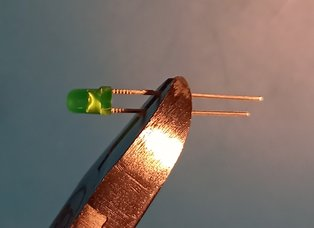
\includegraphics[height=3.5cm]{../pictures/LED4.jpg}
  \captionof{figure}{Schräg abschneiden}
  \label{img:LED4}
  \end{minipage}
\begin{minipage}[t]{0.33\textwidth}
  \centering
  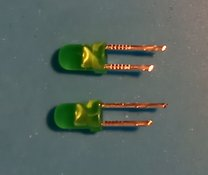
\includegraphics[height=3.5cm]{../pictures/LED5.jpg}
  \captionof{figure}{Lang bleibt lang}
  \label{img:LED5}
\end{minipage}
\begin{minipage}[t]{0.33\textwidth}
  \centering
  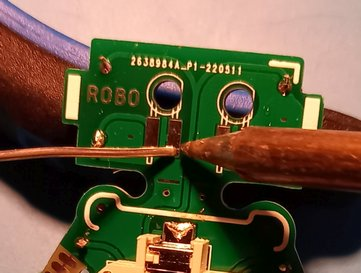
\includegraphics[height=3.5cm]{../pictures/LED6.jpg}
  \captionof{figure}{Pad vorverzinnen}
  \label{img:LED6}
\end{minipage}
\ \\
\begin{minipage}[t]{0.33\textwidth}
  \centering
  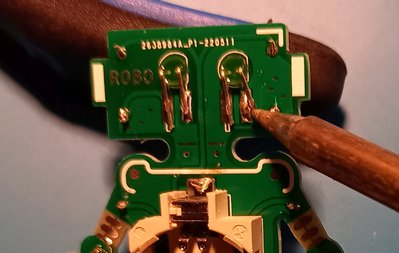
\includegraphics[height=3.5cm]{../pictures/LED7.jpg}
  \captionof{figure}{Rechts verlöten}
  \label{img:LED7}
  \end{minipage}
\begin{minipage}[t]{0.33\textwidth}
  \centering
  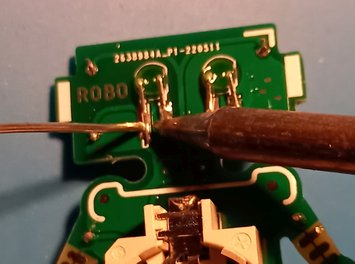
\includegraphics[height=3.5cm]{../pictures/LED8.jpg}
  \captionof{figure}{Links verlöten}
  \label{img:LED8}
\end{minipage}
\subsection{Schritt 6 - Batterie einsetzen}
Die Batterie zuerst oben unter die Metallklammer, danach durchschieben und nach unten drücken, bis sie einrastet.\\
\ \\
\begin{minipage}[t]{0.33\textwidth}
  \centering
  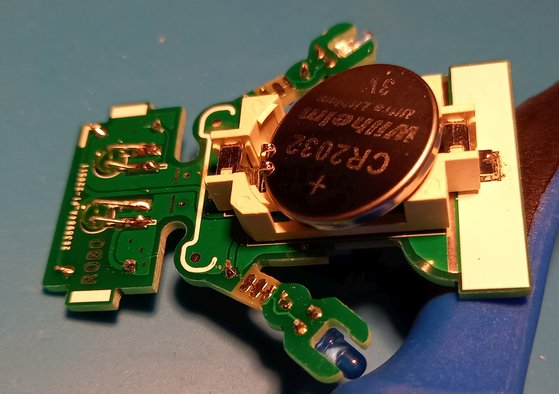
\includegraphics[height=3.5cm]{../pictures/Bat4.jpg}
  \captionof{figure}{Batterie unter die Klammer}
  \label{img:Bat4}
  \end{minipage}
\begin{minipage}[t]{0.33\textwidth}
  \centering
  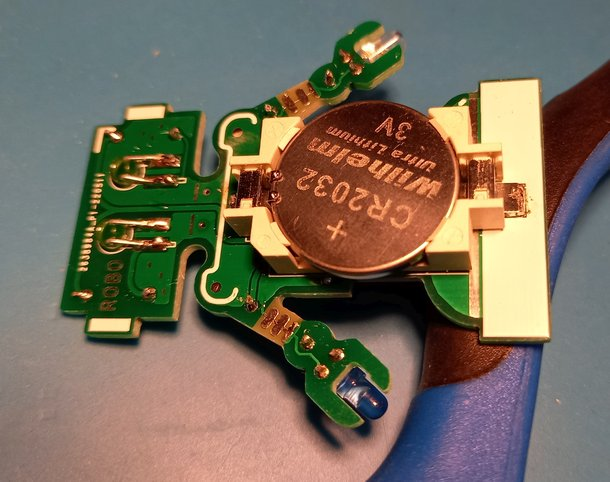
\includegraphics[height=3.5cm]{../pictures/Bat5.jpg}
  \captionof{figure}{Batterie einklippsen}
  \label{img:Bat5}
\end{minipage}
\begin{minipage}[t]{0.33\textwidth}
  \centering
  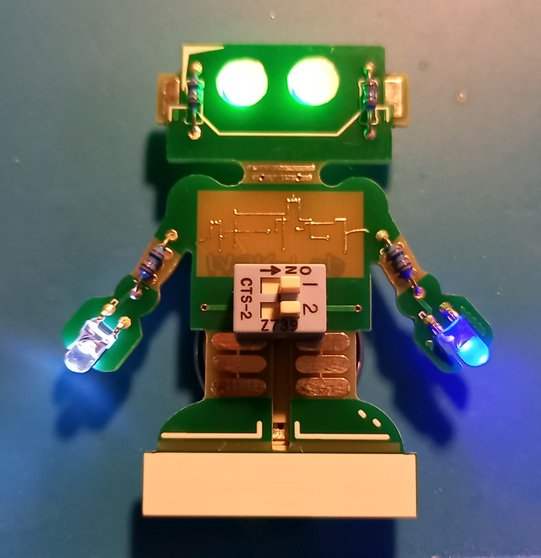
\includegraphics[height=3.5cm]{../pictures/Ready.jpg}
  \captionof{figure}{Schalter nach rechts}
  \label{img:Ready}
\end{minipage}

\end{document}


